% All numerical results are post-production,
% exploratory saved-checkpoint diagnostics run on 24 November 2026.
% Source: scale_diagnostics/summary.json and identity_precision.json.
\subsection{Fixed-weight controls separate geometry from learned representations}
\label{sec:frozen_scale_controls}

To distinguish the immediate effect of geometry from differences acquired during training, we evaluated all 30 classifiers from each of the 9-pixel, 27-pixel fixed-kernel, and 27-pixel dilated-kernel conditions without updating their weights (Fig.~\ref{fig:diagnostics}). Each network was evaluated at patch widths of 9 and 27 pixels and dilations of 1 and 3, with a target occupying one third of the patch width. Noise-free simultaneous-induction probes used identical target and surround colors across geometries, on the RG and BY axes at both surround polarities and contrast magnitude 0.15. Raw signed projection numerators and separately calibrated local, global, and output-logit responses were retained; undefined calibrations remained undefined. These exploratory diagnostics were developed after the production results, with protocols specified before their execution. They are separate from the prespecified primary scale-by-objective endpoint.

With the 9-pixel-trained weights held fixed, the mean local blue--yellow target shift decreased from 0.03013 at width 9 and dilation 1 (95\% seed-bootstrap CI [0.02517, 0.03472]) to 0.00990 at width 27 and dilation 1 ([0.00800, 0.01166]). The paired decrease was $-0.02023$ [$-0.02306$, $-0.01716$], with 28 valid calibrations out of 30 seed blocks. Increasing dilation to 3 at width 27 restored the mean to 0.03013. Both groups trained at 27 pixels showed the same attenuation and restoration (Table~\ref{tab:frozen_scale}). The 27-pixel fixed-kernel weights give a higher mean local response on the shared 9-pixel probe (0.05423) than the 9-pixel-trained weights (0.03013), despite their lower amplitude-based opponent count. This descriptive comparison further separates calibrated functional response from a thresholded weight index. The controls demonstrate an immediate dependence on relative support without requiring differences in learned weights. They do not, by themselves, explain why separately trained networks acquired different weight-based scores.

\begin{table}[htbp]
\centering
\caption{Calibrated local blue--yellow target shifts for fixed saved weights. Positive values indicate assimilation. Columns specify the probe width and convolution dilation. Each row holds weights fixed; $n$ counts valid calibrations among 30 seed blocks and is the same across the three displayed columns. Full seed-bootstrap intervals and red--green, raw, global, and output-logit results are provided with the reproducibility data.}
\label{tab:frozen_scale}
\begin{tabular}{lrrrr}
\hline
Training condition & 9 / $d=1$ & 27 / $d=1$ & 27 / $d=3$ & $n$ \\
\hline
9-pixel, fixed kernel & 0.03013 & 0.00990 & 0.03013 & 28 \\
27-pixel, fixed kernel & 0.05423 & 0.01944 & 0.05423 & 28 \\
27-pixel, dilated kernel & 0.03314 & 0.01098 & 0.03314 & 27 \\
\hline
\end{tabular}
\end{table}

For this architecture, repeating each input pixel into a $3\times3$ block, tripling dilation, and copying weights preserves local feature maps up to repetition. Pointwise nonlinearities and the $1\times1$ convolution commute with repetition, and target/global means are preserved, giving identical representations and outputs in exact arithmetic. Tests on 32 random patches and 14 calibration/induction probes per seed exceeded the specified $10^{-6}$ float32 tolerances in some arrays (maximum logit difference $6.48\times10^{-5}$). A separately specified float64 follow-up passed $10^{-12}$ tolerances for all 30 networks (maximum difference below $1.8\times10^{-14}$), supporting an accumulation-precision explanation. Both outcomes are retained in the release. Independently sampled 27-pixel noise and non-repeated Cornsweet, Mach, and watercolor profiles do not satisfy this exact-input identity.

We also replaced zero padding with replicate or reflect padding after training, using the same test trials for all 90 classifiers. Replicate padding changed 2.82\%, 1.10\%, and 3.37\% of predictions for the 9-pixel, 27-pixel fixed, and 27-pixel dilated groups, respectively. Mean accuracy changes were $+0.500$ percentage points [95\% CI $-0.197$, $+1.193$], $+0.083$ [$-0.283$, $+0.480$], and $+0.360$ [$-0.413$, $+1.097$], using all 30 seeds per group. Reflect padding gave similar results. Local target BY shifts were exactly unchanged, consistent with target receptive fields not reaching the frame, while global representations changed. Thirty intact-context center-only classifiers supplied a negative control: neither padding replacement changed any predicted label or accuracy; logit differences were limited to float32 roundoff. These post-training interventions distinguish local induction from frame-sensitive global readouts. Their effects during learning remain unresolved.

\begin{figure}[p]\centering
\renewcommand{\baselinestretch}{1}\small
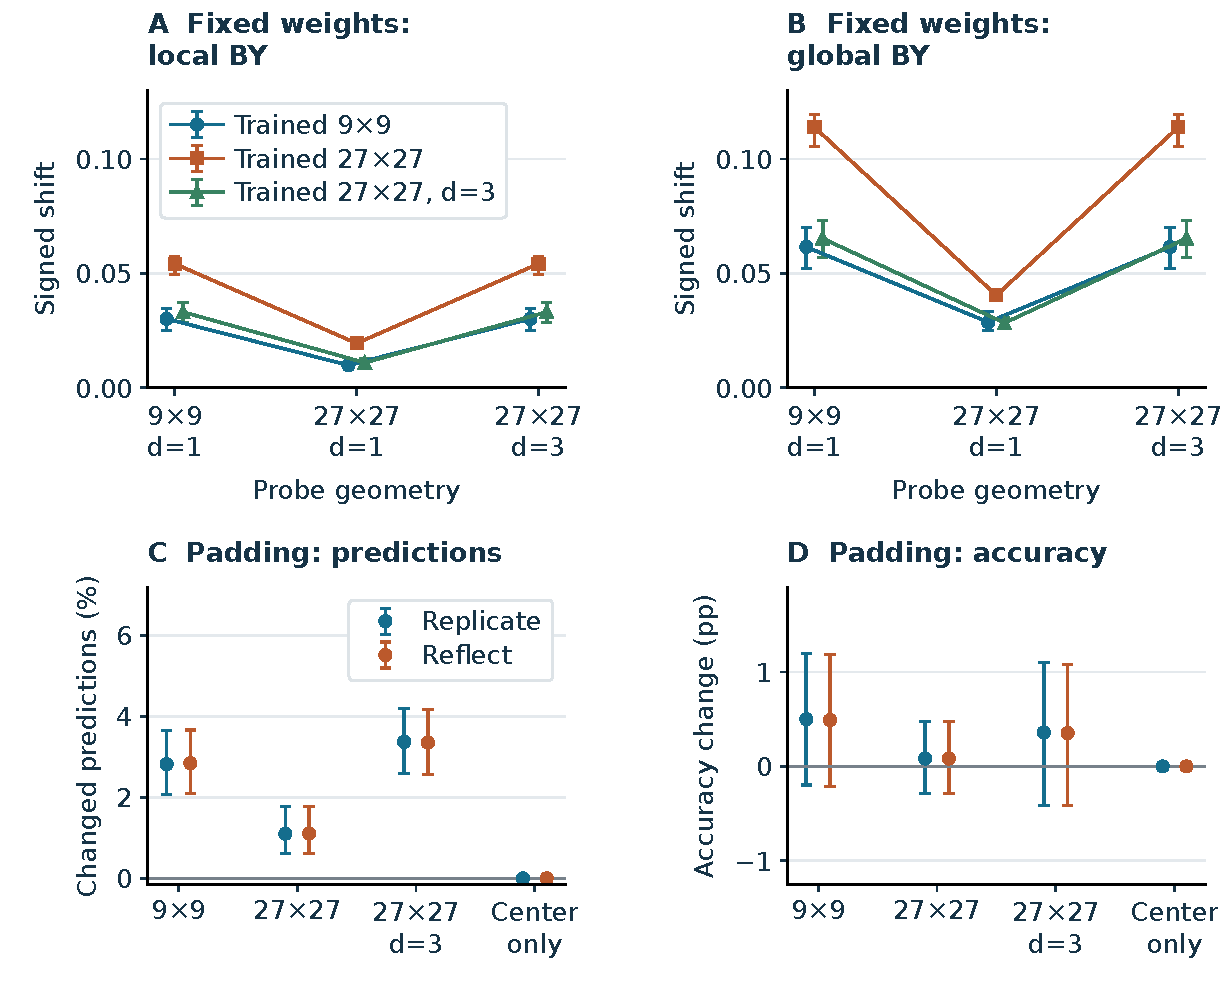
\includegraphics[width=\textwidth,height=0.73\textheight,keepaspectratio]{revision_figures/fixed_weight_controls.pdf}
\caption{Exploratory fixed-weight controls. (A,B) Local and global BY induction across probe width/dilation combinations, with a separate curve for each training geometry. Positive denotes assimilation and negative contrast. Within each curve the weights are unchanged; undefined calibrations are excluded. For training at 9 pixels, 27 pixels with fixed support, and 27 pixels with dilation, valid counts are 28/28/27 locally and 29/28/27 globally. (C,D) Prediction changes and paired accuracy differences when zero padding is replaced after training by replicate or reflect padding. These panels use all 30 seeds per condition; the center-only control uses 27-pixel patches. Intervals are descriptive 95\% seed bootstraps. Local target responses remain unchanged by padding replacement, while some global predictions change.}\label{fig:diagnostics}
\end{figure}
